\edef\mychapter{Complex Numbers}
\edef\mychapterdate{July 2, 2024}

\chapter{\mychapter}
\section{Polar Coordinates}
\subsection{Polar Plane}
In this section, I'm going to try to introduce you to a new way of plotting.
Throughout your entire math career thus far, you may have only been exposed to one type of coordinate system: the Cartesian plane.
But here, we are going to explore ways we can plot things on a graph that don't have an $x$ or a $y$ coordinate.

\begin{figure}
\centering
	\begin{tikzpicture}[scale=.6]
		\coordinate (O) at (0,0);

		\draw[gray, thin, dashed] (O) circle (1);
		\draw[gray, thin, dashed] (O) circle (2);
		\draw[gray, thin, dashed] (O) circle (3);
		\draw (O) circle (4);

		\draw[thick, <->] (-5,0) -- (5,0) coordinate (P);
		\draw[thick, <->] (0,-5) -- (0, 5);

		\node[above, fill=white] (a) at (4.4,0) {$0$};
		\node[right, fill=white] (b) at (0,4.4) {$\frac{\pi}{2}$};
		\node[above, fill=white] (c) at (-4.4,0) {$\pi$};
		\node[right, fill=white] (d) at (0,-4.4) {$\frac{3\pi}{2}$};

		\node[fill=white] (e) at (3.2,3.2) {$\frac{\pi}{4}$};
		\node[fill=white] (f) at (-3.2,3.2) {$\frac{3\pi}{4}$};
		\node[fill=white] (g) at (-3.2,-3.2) {$\frac{5\pi}{4}$};
		\node[fill=white] (h) at (3.2,-3.2) {$\frac{7\pi}{4}$};

		\draw[red,thick] (O) -- (2,3) node[midway, black, left] {$r$};
		\filldraw (2,3) coordinate (A) circle (0.1);
		\pic["$\theta$", draw, ->, black, thick, angle radius=1cm] {angle = P--O--A};
	\end{tikzpicture}
	\caption{}
	\label{fig:polar-intro}
\end{figure}

First, let's define polar coordinates. Like cartesian coordinates, a polar coordinate is also written as an ordered pair, except with the variables $r$ and $\theta$, where $r$ is the distance from the \textbf{pole}, or origin, and $\theta$ is the angle that a ray connecting the pole and point makes with the polar axis, as seen in figure \eqref{fig:polar-intro}.
Normally, we set the polar axis as the positive $x$ axis and let positive angles open counterclockwise.
Since an angle of $2\pi$ is congruent to an angle of $0$, the consequence of using an angle to label a point is that there are infinitely many ordered pairs that we can use to represent a position.
For this reason, we typically restrict $\theta\in(-\pi,\pi]$. The choice we make here is arbitrary, so we could have chosen any interval we'd like, so long as every angle on the plane is reached.
But even still, there are multiple choices of ordered pairs that would label the point.
Let's illustrate this fact in the next example.

\begin{ex}
	For this example, let's find all the possible ways we can label the point $\paren{2,\frac{\pi}{3}}$ given $\theta\in(-\pi,\pi]$.
	First, I've plotted this point in figure \eqref{fig:plot-point}.
	\begin{figure*}
	\centering
	\begin{tikzpicture}[scale=.6]
		\coordinate (O) at (0,0);

		\draw[gray, thin, dashed] (O) circle (1);
		\draw[gray, thin, dashed] (O) circle (2);
		\draw[gray, thin, dashed] (O) circle (3);
		\draw (O) circle (4);

		\draw[thick, <->] (-5,0) -- (5,0) coordinate (P);
		\draw[thick, <->] (0,-5) -- (0, 5);

		\node[above, fill=white] (a) at (4.4,0) {$0$};
		\node[right, fill=white] (b) at (0,4.4) {$\frac{\pi}{2}$};
		\node[above, fill=white] (c) at (-4.4,0) {$\pi$};
		\node[right, fill=white] (d) at (0,-4.4) {$\frac{3\pi}{2}$};

		\node[fill=white] (e) at (3.2,3.2) {$\frac{\pi}{4}$};
		\node[fill=white] (f) at (-3.2,3.2) {$\frac{3\pi}{4}$};
		\node[fill=white] (g) at (-3.2,-3.2) {$\frac{5\pi}{4}$};
		\node[fill=white] (h) at (3.2,-3.2) {$\frac{7\pi}{4}$};

		\filldraw (1,1.732) circle (0.1) node[right, fill=white, xshift=0.2cm] {$\paren{2,\frac{\pi}{3}}$};
		\draw[->,red,thick] (O) -- (0.92,1.632) coordinate (A);
		\pic["$\frac{\pi}{3}$", draw, ->, black, thick, angle radius=.8cm] {angle = P--O--A};
	\end{tikzpicture}
	\caption{}
	\label{fig:plot-point}
	\end{figure*}
	Because of the way we defined $\theta$, as we sweep around the circle, with a radius of $2$, $\frac{\pi}{3}$ is the only time we hit our desired point.
	But since there aren't any restrictions on $r$, we can allow $r$ to be negative. What this would mean is that instead of moving in the direction of the ray defined by the angle, we would go in the opposite direction.
	\begin{figure*}
	\centering
	\begin{tikzpicture}[scale=.6]
		\coordinate (O) at (0,0);
		\coordinate (B) at (0.92,1.632);

		\draw[gray, thin, dashed] (O) circle (1);
		\draw[gray, thin, dashed] (O) circle (2);
		\draw[gray, thin, dashed] (O) circle (3);
		\draw (O) circle (4);

		\draw[thick, <->] (-5,0) coordinate (Q) -- (5,0) coordinate (P);
		\draw[thick, <->] (0,-5) -- (0, 5);

		\node[above, fill=white] (a) at (4.4,0) {$0$};
		\node[right, fill=white] (b) at (0,4.4) {$\frac{\pi}{2}$};
		\node[above, fill=white] (c) at (-4.4,0) {$\pi$};
		\node[right, fill=white] (d) at (0,-4.4) {$\frac{3\pi}{2}$};

		\node[fill=white] (e) at (3.2,3.2) {$\frac{\pi}{4}$};
		\node[fill=white] (f) at (-3.2,3.2) {$\frac{3\pi}{4}$};
		\node[fill=white] (g) at (-3.2,-3.2) {$\frac{5\pi}{4}$};
		\node[fill=white] (h) at (3.2,-3.2) {$\frac{7\pi}{4}$};

		\filldraw (1,1.732) circle (0.1) node[right, fill=white, xshift=0.2cm] {$\paren{2,\frac{\pi}{3}}$};
		\draw[->,purple, thick] (O) -- (-2.5,-4.330) coordinate (A);
		\draw[->,red,dashed] (O) -- (0.92,1.632);
		\pic["$\theta$", draw, <-, black, thick, angle radius=1cm] {angle = A--O--P};
		\pic["$\frac{\pi}{3}$", draw, ->, black, thick, angle radius=.8cm] {angle = Q--O--A};
		\pic["$\frac{\pi}{3}$", draw, ->, black, thick, angle radius=.8cm] {angle = P--O--B};
	\end{tikzpicture}
	\caption{}
	\label{fig:re-plot-point}
	\end{figure*}
	As in figure \eqref{fig:re-plot-point}, if we draw a ray opposite of our original ray, and use that angle, we can use that angle to label our point. In this case, we notice the angle of our new ray with the $-x$-axis is $\frac{\pi}{3}$, since the red line and $x$-axis form vertical angles, by doing a bit of geometry, we find our angle is $-\frac{2\pi}{3}$, hence the other way we can label this point is $(-2,\frac{2\pi}{3})$.
\end{ex}

\subsection{Converting Between Polar and Cartesian}
As you might have already suspected, all of this polar stuff is reminiscent of trig.
As one might expect, we can leverage trig to convert between Cartesian coordinates and polar.

\begin{theorem}
Let $(r,\theta)$ be a point in polar coordinates, then the corresponding point in Cartesian coordinates can be given as $(r\cos(\theta),r\sin(\theta))$. \qed
\label{thm:poletocart}
\end{theorem}
This theorem comes directly from the definition of $\cos(x)$ and $\sin(x)$ by multiplying the circle by a factor of $r$. Using this, we can now try to convert equations plotted in polar, into equations we can plot in Cartesian coordinates (or vice versa).

\begin{ex}
	Let's convert $r=2\sin\theta$ to Cartesian to identify the shape of this curve.
	Multiplying $r$ on both sides gives
	$$r^2=2r\sin\theta.$$
	Since we know
	$$x=r\cos\theta \jand y=r\sin\theta,$$
	that extra $r$ term allows us to substitute out the $r\sin\theta$ term for $y$, therefore,
	$$r^2=2y.$$
	Moreover, $r$ is simply the distance to the origin, using Pythagoras' theorem,
	$$r=\sqrt{x^2+y^2}.$$
	Making this substitution, we have
	$$x^2+y^2=2y.$$
	Then, rearranging the equation and completing the square allows us to get
	$$x^2+y^2-2y=0$$
	$$x^2+y^2-2y+1=1$$
	$$x^2+(y-1)^2=1.$$
	This is simply a unit circle centered at $(0,1)$.
\end{ex}

\begin{ex}
	In this example, let's find the corresponding Cartesian form of the equation
	$$r=\frac{6}{\cos\theta+3\sin\theta}.$$
	Since the trig functions in the denominator lack the factor of $r$ that allows us to easily substitute them for $x$ and $y$, we can divide both sides by $r$ to allow for this.\footnote{Since the only way for $r$ to be 0 is if the numerator is 0. We know this is not possible since the numerator is a non-zero constant.}
	Therefore,
	$$1=\frac{6}{r\cos\theta+3r\sin\theta}$$
	$$1=\frac{6}{x+3y}$$
	$$x+3y=6$$
	hence we conclude this is a line with a slope of $-\frac{1}{3}$ with a $y$-intercept at $(0,2)$.
\end{ex}

\section{Complex Numbers}
\subsection{Polar Form}
Similar to coordinates in a plane, complex numbers also have a corresponding polar form. But before we examine that, we must define an operation that will be key to defining polar complex numbers.

I've mentioned that the complex numbers are not an ordered set, but similar to the real numbers, complex numbers have this notion of distance.
To describe the distance, we use the following.

\begin{define}
	Let the absolute value (modulus) be defined as
	$$|z|=\sqrt{z\bar{z}}$$
\end{define}

We know that $z\bar{z}$ is always positive, from a previous lesson, thus this definition makes $|z|\ge 0$, if we take the square root to be positive.
This definition, in reality, is quite arbitrary: there are many other ways we could have chosen to define this, as long as they satisfy a certain set of criteria.
But we chose this definition since it allows our complex plane to be a plane and agrees with our other definitions of distance in a Euclidean plane.

Now that we have a method of finding the distance from any complex number to the origin, we also need an operation that measures the angle a complex number makes with the positive real axis.

\begin{define}
	Let $\arg: \complex \to \real$ be defined as a multivalued function where $\arg(z)$ returns the argument (angle with respect to the positive real axis) of $z$.
\end{define}

We technically could've used $\tan^{-1}\paren{\frac{b}{a}}$ (and in practice, we will use $\tan^{-1}\paren{\frac{b}{a}}$ to compute $\arg(z)$).
However, $\tan^{-1}\paren{\frac{b}{a}}$ is only defined onto $(-\frac{\pi}{2}, \frac{\pi}{2})$.
Thus, we define $\arg(z)$, which fixes this problem.
However, in general, $\arg(z)$ is a \textbf{multivalued} function, so this is not a function that we defined in Lesson 2 (in particular, this wouldn't be well-defined).
Instead, for any given complex number, it outputs an infinite number of angles.
For this reason, we typically restrict the function to only output onto the interval $(-\pi,\pi]$, which forces $\arg(z)$ to only output one value.
We call this the \textbf{principle argument} and typically denote this corestricted function as $\text{Arg}(z)$.

Now we can define polar complex numbers.
By the definitions, for each complex number $a+ib$, we can associate it with the point $(|z|,\text{Arg}(z))$ in polar coordinates.
By theorem \eqref{thm:poletocart}, we have
$$z=|z|(\cos(\text{Arg}(z))+i\sin(\text{Arg}(z)))$$
We will shorthand this by simply writing
$$z=|z|\text{cis}(\text{Arg}(z))$$
where
$$\text{cis}(\theta)=\cos(\theta)+i\sin(\theta).$$

\begin{ex} \label{ex:multi-cpx-num}
	In this example, let's see how complex numbers multiply in polar form.
	For $z_1, z_2 \in \cpx$, we have in general
	$$z_1=r_1\text{cis}(\theta_1)$$
	$$z_2=r_2\text{cis}(\theta_2)$$
	where
	$$r_1=|z_1| \jand \theta_1=\text{Arg}(z_1)$$
	$$r_2=|z_2| \jand \theta_2=\text{Arg}(z_2).$$
	Then, performing the multiplication gives
	\begin{align*}
		z_1z_2	&=(r_1\text{cis}(\theta_1)) \cdot (r_2\text{cis}(\theta_2)) \\
				&=r_1r_2(\cos(\theta_1)+i\sin(\theta_1))(\cos(\theta_2)+i\sin(\theta_2)) \\
				&=r_1r_2(\cos(\theta_1)\cos(\theta_2)-\sin(\theta_1)\sin(\theta_1)+i\cos(\theta_1)\sin(\theta_2)+i\sin(\theta_1)\cos(\theta_2))
	\end{align*}
	Then, using the cosine and sine sum identities, we have
	\begin{align*}
		&=r_1r_2(\cos(\theta_1+\theta_2)+i\sin(\theta_1+\theta_2)) \\
		&=r_1r_2\text{cis}(\theta_1+\theta_2)
	\end{align*}
\end{ex}

Notice, in the example, we have
$$\text{cis}(\theta_1)\text{cis}(\theta_2) = \text{cis}(\theta_1 + \theta_2).$$
This means $\text{cis}(\theta)$ acts like an exponential as described in the previous lesson.
Observe, the function $\phi: \cpx \to \cpx$ defined via $\phi(x+iy) := e^x\text{cis}(y)$, is clearly continuous and
\begin{align*}
	\phi(x_0+iy_0)\phi(x_1+iy_1) 	&= e^{x_0}\text{cis}(y_0)e^{x_1}\text{cis}(y_1)\\
									&= e^{x_0+x_1}\text{cis}(y_0+y_1)\\
									&= \phi((x_0+x_1)+i(y_0+y_1)).
\end{align*}
Since $\phi(1)=e$, we have that $\phi$ is an exponential with base $e$.
We will take $\phi$ as the definition of the complex exponential, which we will denote $e^{x+ib}$, which is sometimes also known as Euler's Theorem.\footnote{
	While this allows us to take exponentials of arbitrary complex numbers, we will, however, only consider exponentials with \textit{positive real} base.
	This is because generally complex exponentials with a base other than $e$ are of little use, and it comes with complications since these functions are generally multivalued.
}
This formula also gives us a more compact way to denote the polar forms of complex numbers, namely
$$z=|z|e^{i\arg(z)}.$$
Now, with this, we can use the properties that we defined for exponentials to perform complex multiplication and division.\footnote{
	Note, not every property of real exponentials translates to complex exponentials, namely, in general ${e^{z}}^w \neq e^{zw}$ (This is only true when $w$ is an integer).
	The only properties we definitely have are that $e^{w}e^{v}=e^{w+v}$ and immediate corollaries of this.
}

\begin{remark}
	From this definition alone, it is not at all clear that this is the unique complex exponential, and in fact, with our definition of the exponential alone, this function is \textit{not unique} (consider the function defined $\phi(x+iy)=e^x\text{cis}(ky)$ for any real $k$).
	To ensure uniqueness, we give an additional criterion, namely, the exponential must be locally linear at every point, or more explicitly, for every $z_0\in \cpx$, $\phi(z-z_0) \approx a(z-z_0)+\phi(z_0)$ for points sufficiently close to $z_0$.
	For a real function $f$, this condition is exactly the statement that at any $x\in\mathcal D$, there exists a line that runs tangent to the plot of $f$ at $x$ (check that polynomial functions, trig functions, etc.,  all have this property, thus making this a reasonable condition).

	Given this requirement, we can make a few observations:
	For a small change in the input represented by the quantity $z-z_0$, we wish to know how this change affects the output of $\phi$, in particular, we wish to examine the formula
	$$\phi(z)-\phi(z_0).$$
	From before, we established our desire for $\phi$ to be locally linear, since $z-z_0$ is very small, we give the approximation\footnotemark
	$$\phi(z)-\phi(z_0) \approx (az+\phi(z_0))-(az_0+\phi(z_0)) = a(z-z_0).$$
	\footnotetext{We use the same constant $a$ since $z$ and $z_0$ are assumed to be very close, thus we assume they share the same linear approximation.}
	As we see from example \eqref{ex:multi-cpx-num}, the argument of the product of two complex numbers is the sum of the arguments of the multiplicands.
	Since the argument of $a$ is constant, for any $z$ sufficiently close $z_0$, $z-z_0$ is rotated by the same angle by $\phi$.
	In particular, for any two $z, z'$ sufficiently close to $z_0$, then angle between $\phi(z)-\phi(z_0)$ and $\phi(z')-\phi(z_0)$ is equal to the angle between $z-z_0$ and $z'-z_0$.

	In the case when $\phi$ is the exponential, if $z-z_0$ is real, we have
	$$\phi(z)=\phi^{z_0}\phi(z-z_0) = \phi(z_0)e^{z-z_0},$$
	where the last equality follows from the fact that we want $\phi$ to be an extension of $e^x$ to the complex numbers.
	Since $e^{z-z_0}$ is real, we see if $z-z_0$ is real, the result on $\phi$ is a shift towards or away from the origin, which is represented by the blue arrow in figure \eqref{fig:cpx-exp}.
	However, if $z-z_0$ were completely imaginary, since the imaginary axis is perpendicular to the real axis, the effect on $\phi$ must be a shift perpendicular to the radial direction as shown by the magenta arrow in figure \eqref{fig:cpx-exp}.
	The only way for this to be true is if the exponential of imaginary numbers generate \textit{rotations} around the origin of the complex plane, which the definition $\phi(iy)=\text{cis}(y)$ encodes.
	This shows that the exponential of imaginary numbers must result in \textit{rotations} around the origin.\footnote{Special thanks to ziggurism for the inspiration for this explanation. The original post can be accessed at \href{https://math.stackexchange.com/a/2503016}{https://math.stackexchange.com/a/2503016}.}

	\begin{figure*}
	\centering
	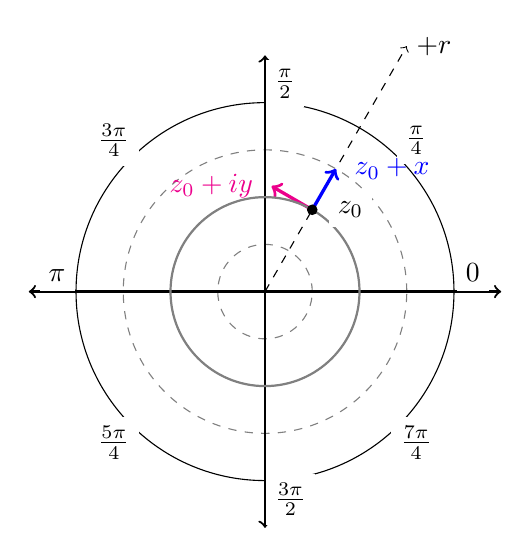
\begin{tikzpicture}[scale=0.6]
		\coordinate (O) at (0,0);

		\draw[gray, thin, dashed] (O) circle (1);
		\draw[gray, thin, dashed] (O) circle (2);
		\draw[gray, thin, dashed] (O) circle (3);
		\draw (O) circle (4);

		\draw[thick, <->] (-5,0) -- (5,0) coordinate (P);
		\draw[thick, <->] (0,-5) -- (0, 5);

		\node[above, fill=white] (a) at (4.4,0) {$0$};
		\node[right, fill=white] (b) at (0,4.4) {$\frac{\pi}{2}$};
		\node[above, fill=white] (c) at (-4.4,0) {$\pi$};
		\node[right, fill=white] (d) at (0,-4.4) {$\frac{3\pi}{2}$};

		\node[fill=white] (e) at (3.2,3.2) {$\frac{\pi}{4}$};
		\node[fill=white] (f) at (-3.2,3.2) {$\frac{3\pi}{4}$};
		\node[fill=white] (g) at (-3.2,-3.2) {$\frac{5\pi}{4}$};
		\node[fill=white] (h) at (3.2,-3.2) {$\frac{7\pi}{4}$};

		\draw[->,black, dashed] (0,0) -- (3, 5.19600) node[right] {$+r$};
		\draw[->,blue, very thick] (1,1.732) -- (1.5, 2.59800) node[right, xshift=0.1cm] {$z_0+x$};
		\draw[->,magenta, very thick] (1,1.732) -- (0.139, 2.232) node[left, xshift=-0.1cm] {$z_0+iy$};

		\draw[gray, thick] (O) circle (2);

		\filldraw (1,1.732) coordinate (z) circle (0.1) node[right, fill=white, xshift=0.2cm] {$z_0$};
	\end{tikzpicture}
	\caption{}
	\label{fig:cpx-exp}
	\end{figure*}

	However, this doesn't quite answer why we can't have $\phi(iy)=\text{cis}(ky)$.
	The answer to this lies in how the values of $k$ affects the \text{rate of change} of $\phi$.
	As we vary $k$, the rate of change of the imaginary part changes since $k$ corresponds to the rate at which we trace around the circle.
	To ensure $\phi$ is locally linear, we require that the rate of change of $\text{cis}(ky)$ agree with the rate of change of $e^x$.
	In particular, this uniformity requires $k=1$.
	A more precise proof of this fact requires an understanding of complex analysis; thus, we will conclude our discussion here.
\end{remark}

\begin{theorem}
	If $z\in\complex$, then
	$$\bar{z}=|z|e^{-i\arg(z)}$$
\end{theorem}
\begin{proof}
	Let $r=|z|$ and $\theta=\arg(z)$, where $\theta$ is any choice of $\arg(z)$.
	Then
	$$z=re^{i\theta}=r(\cos(\theta)+i\sin(\theta))$$
	For $\bar{z}$,
	$$\bar{z}=r(\cos(\theta)-i\sin(\theta))$$
	Then, using the odd and even properties of trig functions:
	$$\bar{z}=r(\cos(-\theta)+i\sin(-\theta)$$
	$$=re^{-i\theta}$$
\end{proof}

\subsection{Roots of Numbers}
Our next order of business is to construct a manner in which we take $n$-roots.
Taking $n$-root of $z_0$ equates to finding the roots of the equation $z^n-z_0=0$.
As mentioned before, for complex numbers, this equation has exactly $n$ roots.
In this section, we will explore ways to compute these roots and, in the process, show that these roots are necessarily unique.

\begin{ex}
	Let's find the $n$-root of $z_0=r_0e^{i\theta_0}$ in general.
	Thus, we wish to find a complex number which we denote as $z=re^{i\theta}$ such that
	$$z_0=(z)^n=(re^{i\theta})^n=re^{in\theta}.$$
	Observe, $e^{2\pi k i} = 1$ for any $k\in \integ$, thus
	$$r_0e^{i\theta_0}=r_0e^{i\theta_0}e^{2\pi i k} = r_0e^{i\theta_0 + 2\pi i k}.$$
	We can solve for $r$ and $\theta$ by comparing to the modulus and argument of $z_0$.
	Thus, we require
	$$r_0 = r^n, \quad \theta_0 +2\pi k= n\theta.$$
	We can solve for $r$ using the $n$-root for real numbers, which we denote $r = \sqrt[n] r_0$.\footnote{We let $\sqrt[n] r_0$ output only the positive result for any real number $r$.}
	The equality derived from the arguments gives $\theta = \frac{\theta_0}{n}+\frac{2\pi k}{n}$.
	Notice, the formula for $\theta$ gives $n$ distinct angles as depicted in figure \eqref{fig:root-of-unity} for $n=4$.
	These angles each generate $n$ unique complex numbers, and one can check that these are each indeed $n$-roots of $z$.


	\begin{figure*}
	\centering
	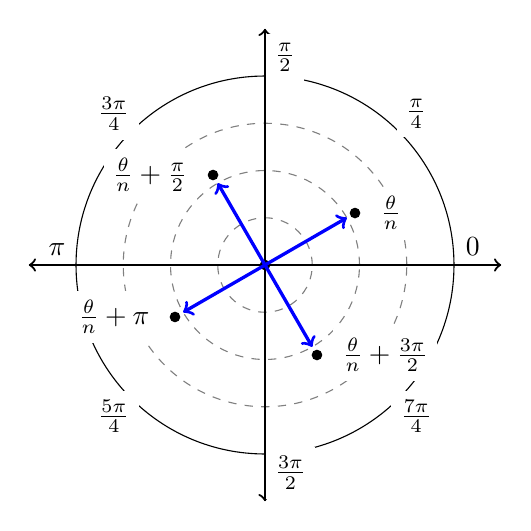
\begin{tikzpicture}[scale=.6]
		\coordinate (O) at (0,0);

		\draw[gray, thin, dashed] (O) circle (1);
		\draw[gray, thin, dashed] (O) circle (2);
		\draw[gray, thin, dashed] (O) circle (3);
		\draw (O) circle (4);

		\draw[thick, <->] (-5,0) -- (5,0) coordinate (P);
		\draw[thick, <->] (0,-5) -- (0, 5);

		\node[above, fill=white] (a) at (4.4,0) {$0$};
		\node[right, fill=white] (b) at (0,4.4) {$\frac{\pi}{2}$};
		\node[above, fill=white] (c) at (-4.4,0) {$\pi$};
		\node[right, fill=white] (d) at (0,-4.4) {$\frac{3\pi}{2}$};

		\node[fill=white] (e) at (3.2,3.2) {$\frac{\pi}{4}$};
		\node[fill=white] (f) at (-3.2,3.2) {$\frac{3\pi}{4}$};
		\node[fill=white] (g) at (-3.2,-3.2) {$\frac{5\pi}{4}$};
		\node[fill=white] (h) at (3.2,-3.2) {$\frac{7\pi}{4}$};

		\filldraw (1.905,1.1) coordinate (z) circle (0.1) node[right, fill=white, xshift=0.2cm] {$\frac{\theta}{n}$};
		\filldraw (-1.1,1.905) coordinate (z) circle (0.1) node[left, fill=white, xshift=-0.2cm] {$\frac{\theta}{n}+ \frac{\pi}{2}$};
		\filldraw (-1.905, -1.1) coordinate (z) circle (0.1) node[left, fill=white, xshift=-0.2cm] {$\frac{\theta}{n}+\pi$};
		\filldraw (1.1, -1.905) coordinate (z) circle (0.1) node[right, fill=white, xshift=0.2cm] {$\frac{\theta}{n}+\frac{3\pi}{2}$};

		\filldraw (0,0) circle (0.1);

		\draw[very thick, blue, ->] (0,0) -- (1.732,1);
		\draw[very thick, blue, ->] (0,0) -- (-1,1.732);
		\draw[very thick, blue, ->] (0,0) -- (-1.732,-1);
		\draw[very thick, blue, ->] (0,0) -- (1, -1.732);

	\end{tikzpicture}
	\caption{}
	\label{fig:root-of-unity}
	\end{figure*}

	By the fundamental theorem of algebra, since the $z^n-z_0$ has at most $n$ distinct roots.
	Thus, the $n$ distinct values which we computed must be the only $n$-roots of $z_0$.
	In particular, we also see that these roots each have multiplicity one.
	If we denote the $n$-root of $z$ as $z^{\frac{1}{n}}$, then we have the formula
	\begin{align*}
		z^{\frac{1}{n}} = \paren{re^{i\theta}}^{\frac{1}{n}} 	&= \paren{re^{i\theta+2\pi i k}}^{\frac{1}{n}} \\
																&= \sqrt[n] r e^{i \frac{\theta}{n} + \frac{2\pi i k}{n}}, \quad \text{for } k \in \{0, ..., n-1\}
	\end{align*}
\end{ex}

\begin{ex}
	With the formula we computed before, let's compute the cube root of $z=1+i$.
	First, we compute the modulus of $z$:
	$$|z|=\sqrt{(1+i)(1-i)}=\sqrt{2}$$
	Then for the principal argument:
	$$\text{Arg}(z)=\tan^{-1}(1)=\frac{\pi}{4}\footnotemark$$
	\footnotetext{Of course, we check that $tan^{-1}(x)$ output in the right quadrant, or we would need to modify the output.}
	Therefore
	$$z=\sqrt{2}\exp\paren{\frac{i\pi}{4}}$$
	Then, using the formula in the last example:
	$$\sqrt[3]{z}=\sqrt[6]{2}\exp\paren{\frac{i\pi}{4}\cdot\frac{1}{3}+\frac{2i\pi k}{3}} \for k\in\integ$$
	$$=\sqrt[6]{2}\exp\paren{\frac{i\pi}{12}+\frac{2}{3}i\pi k}.$$
	Then, the 3 unique solutions are
	$$\cbrak{\sqrt[6]{2}\exp\paren{\frac{i\pi}{12}},\sqrt[6]{2}\exp\paren{\frac{3i\pi}{4}},\sqrt[6]{2}\exp\paren{\frac{17i\pi}{12}}}$$
\end{ex}
\subsection{Complex Logarithms}
\begin{ex} \label{ex:cpx-log}
	In this example, I'm going to compute a complex logarithm in general. In terms of notation, we typically use $\ln(x)$ to define the natural logarithm in the real sense, and in $\log(z)$ to denote the more general complex logarithm.\footnote{
		We generally don't talk about logarithms for complex variables with arbitrary bases, since it turns out, those are generally less useful and can be replaced simply by dividing by the logarithm of the respective base.
	}
	Thus, since $z=|z|re^{\i\arg(z)}$, by using the definition of the logarithm and its properties:
	$$\log(z)=\log(|z|e^{\i\arg(z)})=\ln(|z|)+\log(e^{i\arg(z)})=\ln(r)+i\arg(z).$$
	Since $\arg(z)$ is a multivalued function, $\log(z)$ too is a multivalued function.
	By taking the principal value, we obtain the formula
	$$\text{Log}(z)=\ln(r)+i\text{Arg}(z).$$
\end{ex}

\begin{remark}
	In example \eqref{ex:cpx-log}, we successfully extend the logarithm to all complex numbers except $0$.
	Even in this extended setting, the logarithm of zero is still ill-defined.
\end{remark}

\begin{ex}
	Now using the above formula, let's compute $\text{Log}(-\sqrt{3}+i)$.
	First, finding the modulus of $z$ we get
	$$|z|=\sqrt{z\bar{z}}=\sqrt{(-\sqrt{3}+i)(-\sqrt{3}-i)}=2$$
	Then computing the principal argument:
	$$\text{Arg}(z)=\tan^{-1}\paren{-\frac{1}{\sqrt{3}}}=\frac{5\pi}{6}\footnotemark$$
	\footnotetext{Make sure we chose the domain for $\tan^{-1}(\theta)$ that outputs in the right quadrant, don't just plug this into a calculator.}
	Therefore,
	$$\text{Log}(z)=\ln(2)+\frac{5i\pi}{6}$$
	or if we expand to all outputs of $\log(z)$,
	$$\log(z)=\ln(2)+\frac{5i\pi}{6}+2i\pi k \for k\in\integ$$
\end{ex}
